\chapter{Hyperparameter optimisation of a classifying neural network}
\label{sec:simpleNN}

The basis od the adversarial neural network is a common neural network trained on signal/background classification.
Before the adversary, second network is added the network is optimised on its own to make sure that its setup is sufficient for the classification task.
During the adversarial training this setup can be updated if the structure is not optimised for the additional task of a model independent of systematics.

This chapter describes the hyperparameter optimisation of the first network. The first section deals with the input information.
The second section explains the choice of the architecture followed by the setup of the optimiser.
Lastly regularisation of the network is described.

\section{The input variables}

got bdt variables

compared to simple kinematic

\begin{figure}
	\centering
	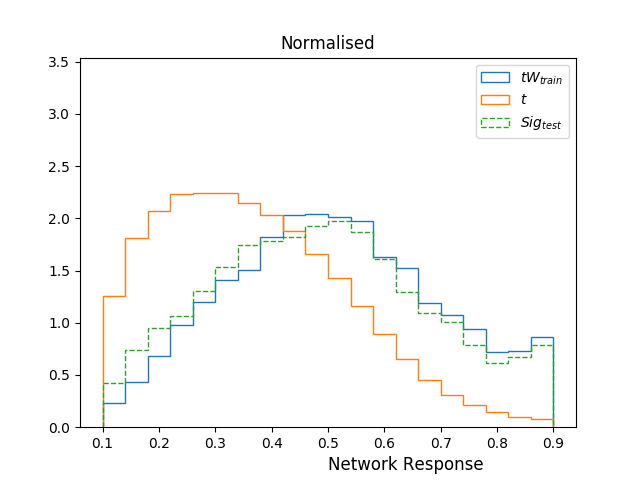
\includegraphics[width=\figwidth]{figures_simpleNN/test_simple.png}
\end{figure}



\section{The network architecture}

The architecture of the neural network is formed by its nodes and layers. The choice of the architecture is nontrivial and as a lot of aspect's of machine learning not an exact science.
However, one can make some assumptions about the appropriate architecture.
First of all the complexity of the model should about match the complexity of the task assigned. Although it usually is not trivial to find an estimator for a task's complexity and even less to match it to a certain architecture a test series often lads to a good estimate.
Both the depth and the overall size of the model play a role. The depth defines how often the input is processed during the network. The number of nodes is the number of features that can be kept during each step of processing.

In general an architecture that is too deep and wide will pick up too many features too fast and overtrains before it gets to a good minimum. This can be seen in an early divergence between the training loss and the validation loss. An architecture too simple is not able to pick up the features of the task at all and is not learning at all. The loss stays constant or changes very slowly.

In this work a testseries was performed, training a network for a wide range combinations of nodes and layers. For the sake of simplicity the number of nodes per layer was kept constant during each training. Two variables were then plotted against the size of the architecture. First the overall smallest loss the model achieved during the training was plotted. The other variable was the minimal difference between the training and the validation loss. To keep it simple the complexity of the architecture was defined as the product of nodes and layers. These are certainly not the most sophisticated indicators for the model's complexity and its performance. Nonetheless the plots show that region of good performance exists which was chosen for this analysis.

The good region lays between about x and y layers and x and y nodes each

Furthermore the activation function for the hidden layer is elu
the activation function 

\section{Setup of the optimisation}

\section{Regularisation}